
%----------------------------------------------------------------------------------------
%	PACKAGES AND OTHER DOCUMENT CONFIGURATIONS
%----------------------------------------------------------------------------------------

\documentclass[paper=a4, fontsize=11pt]{scrartcl} % A4 paper and 11pt font size

\usepackage[utf8]{inputenc}
\usepackage[T1]{fontenc} % Use 8-bit encoding that has 256 glyphs
\usepackage[polish]{babel} % English language/hyphenation
\usepackage{amsmath,amsfonts,amsthm} % Math packages

\usepackage{babelbib}

\usepackage{graphicx}
\usepackage{sectsty} % Allows customizing section commands
%\allsectionsfont{\centering \normalfont\scshape} % Make all sections centered, the default font and small caps
\usepackage{hyperref}

\usepackage{fancyhdr} % Custom headers and footers
\pagestyle{fancyplain} % Makes all pages in the document conform to the custom headers and footers
\fancyhead{} % No page header - if you want one, create it in the same way as the footers below
\fancyfoot[L]{} % Empty left footer
\fancyfoot[C]{} % Empty center footer
\fancyfoot[R]{\thepage} % Page numbering for right footer
\renewcommand{\headrulewidth}{0pt} % Remove header underlines
\renewcommand{\footrulewidth}{0pt} % Remove footer underlines
\setlength{\headheight}{13.6pt} % Customize the height of the header

\numberwithin{equation}{section} % Number equations within sections (i.e. 1.1, 1.2, 2.1, 2.2 instead of 1, 2, 3, 4)
\numberwithin{figure}{section} % Number figures within sections (i.e. 1.1, 1.2, 2.1, 2.2 instead of 1, 2, 3, 4)
\numberwithin{table}{section} % Number tables within sections (i.e. 1.1, 1.2, 2.1, 2.2 instead of 1, 2, 3, 4)

\setlength\parindent{0pt} % Removes all indentation from paragraphs - comment this line for an assignment with lots of text

%----------------------------------------------------------------------------------------
%	TITLE SECTION
%----------------------------------------------------------------------------------------

\newcommand{\horrule}[1]{\rule{\linewidth}{#1}} % Create horizontal rule command with 1 argument of height

\title{	
\normalfont \normalsize 
\textsc{Metody Odkrywania Wiedzy} \\ [25pt] % Your university, school and/or department name(s)
\horrule{0.5pt} \\[0.4cm] % Thin top horizontal rule
\huge Nie-całkiem-naiwny klasyfikator Bayesa \\ % The assignment title
\horrule{2pt} \\[0.5cm] % Thick bottom horizontal rule
\LARGE Dokumentacja końcowa
}%


\author{Mateusz Jamiołkowski, Michał Uziak} % Your name

\date{\normalsize\today} % Today's date or a custom date

\begin{document}

\maketitle % Print the title

%----------------------------------------------------------------------------------------
%	PROBLEM 1
%----------------------------------------------------------------------------------------
\newpage

\tableofcontents

\newpage

\section{Wstęp}

Celem projektu jest implementacja algorytmu budowy sieci bayesowskiej, która będzie uwzględniać zależności między atrybutami klasyfikowanych obiektów. Na podstawie tak zbudowanego modelu zostanie zaimplementowany alogrytm, którego działanie zostanie porównane z dostępnymi modułami klasyfikacji języka R.

\section{Algorytm}
Na podstawie analizy dostępnych materiałów zdecydowano, że budowa sieci bayesowskiej zostanie zaimplementowana z wykorzystaniem drzew TAN (tree-augmented naive Bayesian Network). 

\subsection{Opis działania algorytmu tworzącego sieć bayesowską}



Opis algorytmu tworzenia drzew TAN:
\begin{enumerate}
 \item Obliczenie informacji wzajemnej $I_p(A_i,A_j|C)$ dla każdej pary atrybutów $A_i, A_j$ takich, że $i\neq j $, gdzie 
 $I_p(A_i,A_j|C)= \sum_{c \in C}^{} {P(A_i,A_j,c) \log\frac{P(A_i,A_j|c)}{P(A_i|c)P(A_j|c)} } $ ,$C$ - klasa obiektu.
 
 \item  Budowa grafu zupełnego nieskierowanego, którego wierzchołkami będą atrybuty $A_1,... ,A_n$ natomiast waga krawędzi pomiędzy atrybutami $A_i$ i $A_j$ 		będzie równa $I_p(A_i,A_j)$
 
 \item  Budowa minimalnego drzewa rozpinającego z wykorzystaniem algorytmu Kruskala.
 \item  Stworzenie drzewa skierowanego, poprzez wybór jednego wierzchołka $A_p$. Kierunek każdej krawędzi w drzewie zostanie tak dobrany, aby, przechodząc zgodnie z kierunkiem krawędzi, odległość od wierzchołka $A_p$ rosła.
 \item Dodanie wierzchołka $C$(reprezentującego klasę obiektu) do drzewa oraz utworzenie krawędzi skierowanych “od” wierzchołka $C$ pomiędzy tym wierzchołkiem a już istniejącymi wierzchołkami $A_1,A_2...A_n$.
 
\end{enumerate}

\subsection{Opis konstrukcji klasyfikatora}
Działanie klasyfikatora będzie polegało na wyborze klasy, która jest najbardziej prawdopodobna dla danego zestawu wartości atrybutów. W odróżnieniu od  naiwnego klasyfikatora Bayesa, budowany klasyfikator będzie uwzględniał wzajemne zależności atrybutów. W zbudowanym drzewie krawędź wchodząca do węzła(atrybutu) oznacza zależność od innego węzła(atrybutu). Na rysunku \ref{fig:model_drzewa} przedstawiono przykładowy model drzewa TAN. Zgodnie z przedstawioną zasadą łatwo zauważyć, że atrybut $A_2$ jest zależny od atrybutu $A_1$ oraz klasy $C$.
\begin{figure}[h]
 \centering
 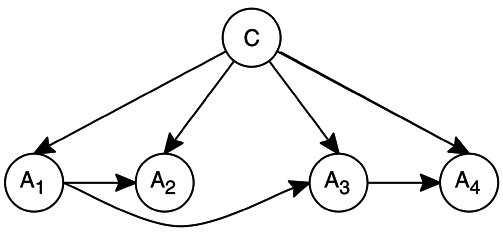
\includegraphics[width=70mm]{model1.png}
 \caption{Przykładowy model drzewa}
 \label{fig:model_drzewa}
\end{figure}

Klasyfikator będzie wyznaczał klasę danego obiektu zgodnie z poniższym wzorem:
\[h(x) = \operatorname*{arg\,max}_{c \in C} P(c|a_1,...,a_n)= \frac{P(c,a_1,a_2,...,a_n)}{P(a_1,a_2,...,a_n)}= 
\frac {P(c) \cdot \prod_{i=1}^{n} {P(a_i|c,a_j)}}{P(a_1,a_2,...,a_n)} \]

Wyrażenie $P(a_i|c,a_j)$ odzwierciedla zależności w zbudowanym drzewie TAN - atrybut $A_i$ jest zależny od $A_j$

Implementacja algorytmu i powyższy opis zostały stworzone na podstawie artykułu \cite{Bayesian_Network_Classifiers}

\section{Implementacja}

W formie pakietu  języka R o nazwie \textit{notSoNaiveBayes} zostały udostępnione następujące funkcje:
\begin{itemize}
 \item \textit{notSoNaiveBayes} - funkcja domyślna, która na podstawie danych uczących buduje model, który jest zwracany jako obiekt języka R.
 \item \textit{predict} - funkcja, która na podstawie modelu uzyskanego w wyniku działania funkcji \textit{notSoNaiveBayes} i wektora (macierzy) atrybutów próbek przypisuje im klasę.
\end{itemize}

Dodatkowo na potrzeby implementacji zostały napisane następujące funkcje:
\begin{itemize}
 \item \textit{buildDirectedTree} - funkcja, która na wejściu przyjmuje graf nieskierowany zakodowany w formie macierzy sąsiedztwa oraz numer wierzchołka grafu, który ma zostać korzeniem drzewa jakie powstanie jako argument wyjściowy tej funkcji.
 \item \textit{kruskal} - jest to implementacja klasycznego algorytmu Kruskala, z jedną różnicą,napisana funkcja szuka maksymalnego drzewa rozpinającego.
\end{itemize}

\section{Testy}

W celu sprawdzenia jakości zbudowanego klasyfikatora jego działanie zostało porównane z innymi algorytmami klasyfikacji dostępnymi w modułach języka R: \\
\begin{itemize}
\item naiwnym klasyfikatorem Bayesa - moduł e1071
\item algorytmem kNN - moduł kknn 
\end{itemize}

Do testów zostaną wykorzystane dane należące do repozytorium Uniwersytetu Kalifornijskiego w Irvine (Machine Learning Repository, University of California, Irvine), dostępne pod adresem: \url{http://archive.ics.uci.edu/ml/datasets.html}.

Zbiory testowe:
\begin{itemize}
\item chess \url{http://archive.ics.uci.edu/ml/datasets/Chess+%28King-Rook+vs.+King-Pawn%29}
\item nursery \url{http://archive.ics.uci.edu/ml/datasets/Nursery}
\item car \url{http://archive.ics.uci.edu/ml/datasets/Car+Evaluation}
\end{itemize}

Testy zostały przeprowadzone za pomocą metody Bootstrap. Dla każdego zbioru danych rozlosowano dwie próbki - uczącą i testową. Algorytmy zostały przetestowane dziesięciokrotnie.

Wynikiem była procentowa jakość klasyfikacji, określona za pomocą funkcji języka R:
\begin{itemize}
\item \textit{confusionMatrix} - dla algorytmów Bayesowskich
\item \textit{simulation} - dla algorytmu knn
\end{itemize}

\section{Porównanie jakości klasyfikacji }

Wykresy przedstawiają porównanie jakości klasyfikacji dla zbiorów testowych. Algorytmy badano kolejno dla losowych danych uczących i testowych.

\begin{table}[t]
\caption{Wyników testów klasyfikacji}
\label{tabela}
\begin{tabular}{|l|l|l|l|l|l|l|l|l|l|}
  \hline 
  Nr próby & \multicolumn{3}{l|}{Car} & \multicolumn{3}{r|}{Nursery} & \multicolumn{3}{l|}{Chess} \\ \hline
  0 & Naive & Not Naive & k-NN  & Naive & Not Naive & k-NN & Naive & Not Naive & k-NN \\ \hline
  1 & 0,8 &	0,95 &0,78 &0,76	&0,85&0,86 & 0,91	&0,94	&0,8\\
  2 & 0,8 &	0,93 &0,75 &0,75&0,84&0,89&0,85&0,92	&0,84\\
  3 &0,82 & 0,94 &0,77&0,76&0,85&0,88&0,9&	0,93&	0,85\\
  4 &0,78 &	0,92	 &0,75&0,76&0,85&0,88&0,85&	0,9&	0,8\\
  5 &0,79 &	0,96 &0,81&0,76&	0,84&	0,87& 0,87&	0,93	&0,83\\
  6 &0,82 & 0,94	 &0,8&0,75&	0,85	&0,88&0,88&	0,93	&0,83\\
  7 &0,78 &	0,94 &0,8&0,73&	0,87	&0,88&0,9	&0,93	&0,8\\
  8 &0,8  &	0,93 &0,78&0,75&0,86&0,89&0,89	&0,94	&0,84\\
  9 &0,8 & 0,95 & 0,78&0,74&0,85&0,88&0,87&	0,93	&0,81\\
  10&0,83& 0,94 &0,83&0,74&0,8&0,87&0,9&	0,93	&0,86\\

  \hline
\end{tabular} 
\end{table}

Poniższe wykresy zawierają dane zamieszczone w tabeli \ref{fig:tabela}

\begin{figure}[h]
 \centering
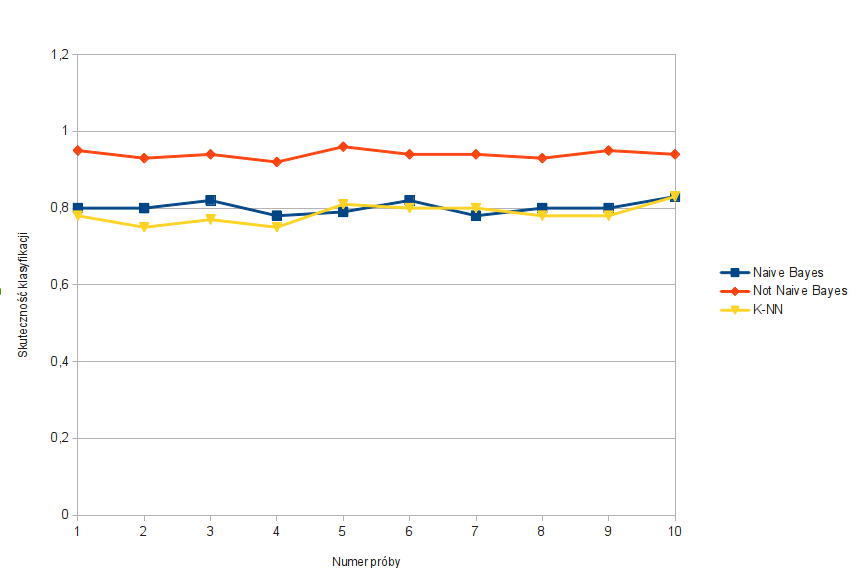
\includegraphics[width=150mm]{car.png}
 \caption{Wyniki dla zbioru testowego car}
 \label{fig:model_drzewa}
\end{figure}

\begin{figure}[h]
 \centering
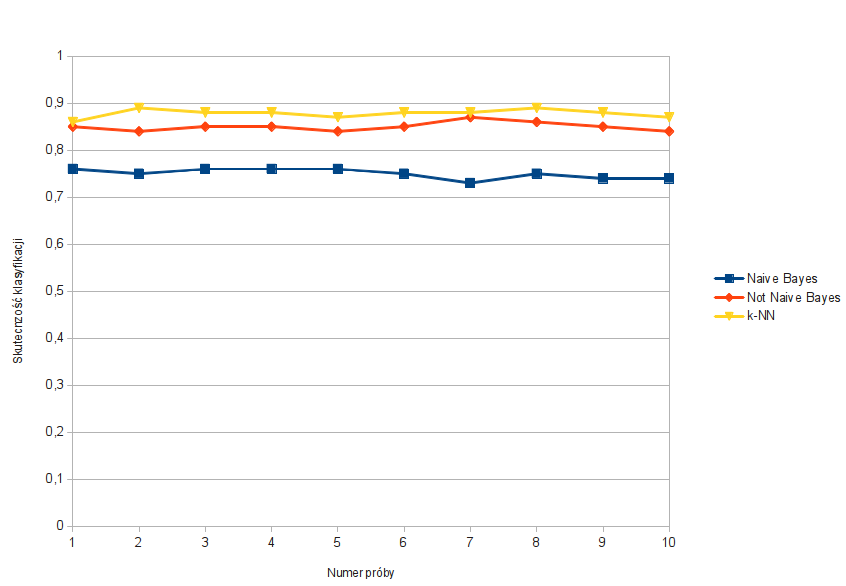
\includegraphics[width=150mm]{nursery.png}
 \caption{Wyniki dla zbioru testowego nursery}
 \label{fig:model_drzewa}
\end{figure}

\begin{figure}[h]
 \centering
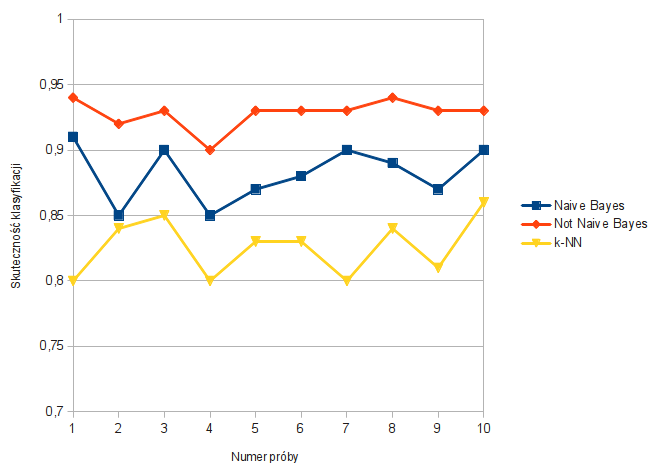
\includegraphics[width=150mm]{chess.png}
 \caption{Wyniki dla zbioru testowego chess}
 \label{fig:model_drzewa}
\end{figure}

Z wykresów widać, że zaimplementowany klasyfikator Bayesowski wykazuje się najlepszą skutecznością działania spośród wszystkich przebadanych algorytmów. 

\section{Wnioski}
Projekt wykazał, że implementacja algorytmu Bayesowskiego, opartego o drzewo TAN, wykazuje większą dokładność klasyfikacji od klasycznego klasyfikatora Bayesowskiego. Algorytm kNN wykazał się lepszą skutecznością od pozostałych modułów dla zbioru nursery. W pozostałych przypadkach jego jakość nie przekraczała poziomu naiwnego klasyfikatora Bayesa.
\newpage

\bibliographystyle{plain}
\bibliography{./biblio.bib} 




\end{document}